\section{基本采样算法}
本节中,我们研究从一个给定的概率分布中生成随机样本的一些简单的方法。
\subsection*{标准概率分布}
首先,我们考虑如何从简单的非均匀分布中生成随机数,假定我们已经有了一个均匀分布的随机数的来源。假设$z$在区间$(0,1)$上均匀分布,我们使用某个函数$f(\cdot)$对$z$的值进行变换,即$y=f(z)$。$y$上的概率分布为
\begin{equation}
\label{suiji}
	p(y)=p(z)\bigg|\frac{\mathrm{d}z}{\mathrm{d}y}\bigg|
\end{equation}
其中,在这种情况下,$p(z)=1$。我们的目标是选择一个函数$f(z)$使得产生出的$y$值具有某种所需的具体的分布形式$p(y)$,对公式$\ref{suiji}$进行积分,我们有
\begin{equation}
	z=h(y)\equiv \int _{-\infty}^{y}p(\hat{y})d\hat{y}
\end{equation}
它是$p(y)$的不定积分,因此$y=h^{-1}(z)$,因此我们必须使用一个函数来对这个均匀分布的随机数进行变换,这个函数是所求的概率分布的不定积分的反函数,如图所示
\begin{center}
	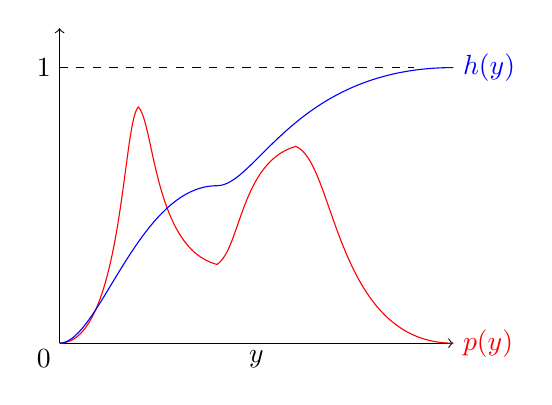
\begin{tikzpicture}
		\draw[->] (0,0) -- (5,0) node at (-0.2,3.5) {$1$};
		\draw[->] (0,0) -- (0,4) node at (-0.2,-0.2){$0$};
		\draw[dashed] (0,3.5) -- (4.5,3.5) node at (2.5,-0.2) {$y$};
		
		\draw[red]  
		(0,0) .. controls (0.8,0) and (0.8,2.8)  ..  (1,3) .. controls (1.2,2.8) and (1.2,1.2) .. (2,1) .. controls (2.3,1.2) and (2.3,2.3) .. (3,2.5) .. controls (3.5,2.3) and (3.5,0) .. (5,0) node[right] {$p(y)$};
		\draw[blue] (0,0) .. controls (0.5,0) and (1,2) .. (2,2) .. controls (2.5,2) and (3,3.5) ..(5,3.5) node[right] {$h(y)$};

	\end{tikzpicture}
\end{center}
\subsection*{拒绝采样}
\subsection*{可调节的拒绝采样}
\subsection*{重要采样}
\subsection*{采样-重要性-重采样}
\subsection*{采样与EM算法}
